\documentclass{beamer}
\usetheme{default}
\useoutertheme{miniframes}
\useinnertheme{circles}
\usepackage{graphicx}
\usepackage{hyperref}
\usepackage{pdfpages}
\usepackage{color}
\usepackage{pgf}

\logo{\pgfputat{\pgfxy(-11, 0)}{\pgfbox[center,base]{
\includegraphics[width=2.5cm]{ANUlogo.png}}}} 

\definecolor{ANUbg}{rgb}{0.2, 0.2, 0.2}
\definecolor{ANUblue}{rgb}{0.56, 0.69, 0.75}
\usecolortheme[named=ANUbg]{structure}

\title{Machine Learning Approaches to Computational Protein Design}


\author{Stephen Zhang}
\addtobeamertemplate{navigation symbols}{}{ \hspace{1em}    \usebeamerfont{footline}%
    \insertframenumber / \inserttotalframenumber }
    

% Let's get started
\begin{document}

\begin{frame}
  \titlepage
\end{frame}

\section{Introduction}

\begin{frame}
    \begin{itemize}
        \item Computational techniques can be applied to the problem of designing orthogonal mutant aaRS that exhibit affinity and specificity for uAAs.
        \item Computational protein design allows for a \textbf{huge reduction of search space} \textit{in silico} $\Rightarrow$ less lab work!
        \item \texttt{Rosetta} is a software package offering a wide range of protein computation protocols $\Rightarrow$ \texttt{EnzymeDesign}
        \item We aimed to use \textbf{machine learning techniques} to address shortcomings of 'na\"ively' using Rosetta output.
    \end{itemize}
\end{frame}

\begin{frame}
    Conventional (na\"ive) protocol:
    \begin{enumerate}
        \item Construct protein model based off crystal structures. Place uAA in binding site, specify mutation sites and catalytic constraints.
        \item Generate mutant candidates using \texttt{Rosetta} \texttt{EnzymeDesign} $\Rightarrow$ \textbf{score factors} for mutants.
        \begin{center}Mutant pose $\to$ $\mathrm{scores}(E_1, E_2, E_3, ...)$\end{center}
        \item Select candidates for \textit{in vitro} screening by applying thresholds or ranking w.r.t several score factors (e.g. total score, ligand binding score), e.g. $\underbrace{\text{total score} > E_0}_{\text{a rectangular constraint!}}$
    \end{enumerate}
\end{frame}

\begin{frame}
    Rectangular constraints
    \begin{center}
    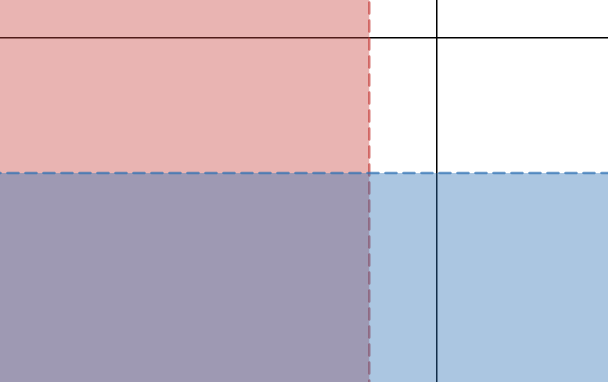
\includegraphics[width=0.8\linewidth]{rectangularconstraints.png}
    \end{center}
\end{frame}

\begin{frame}
    This has significant limitations: boundary between 'good' and 'bad' may be nonlinear! \\
    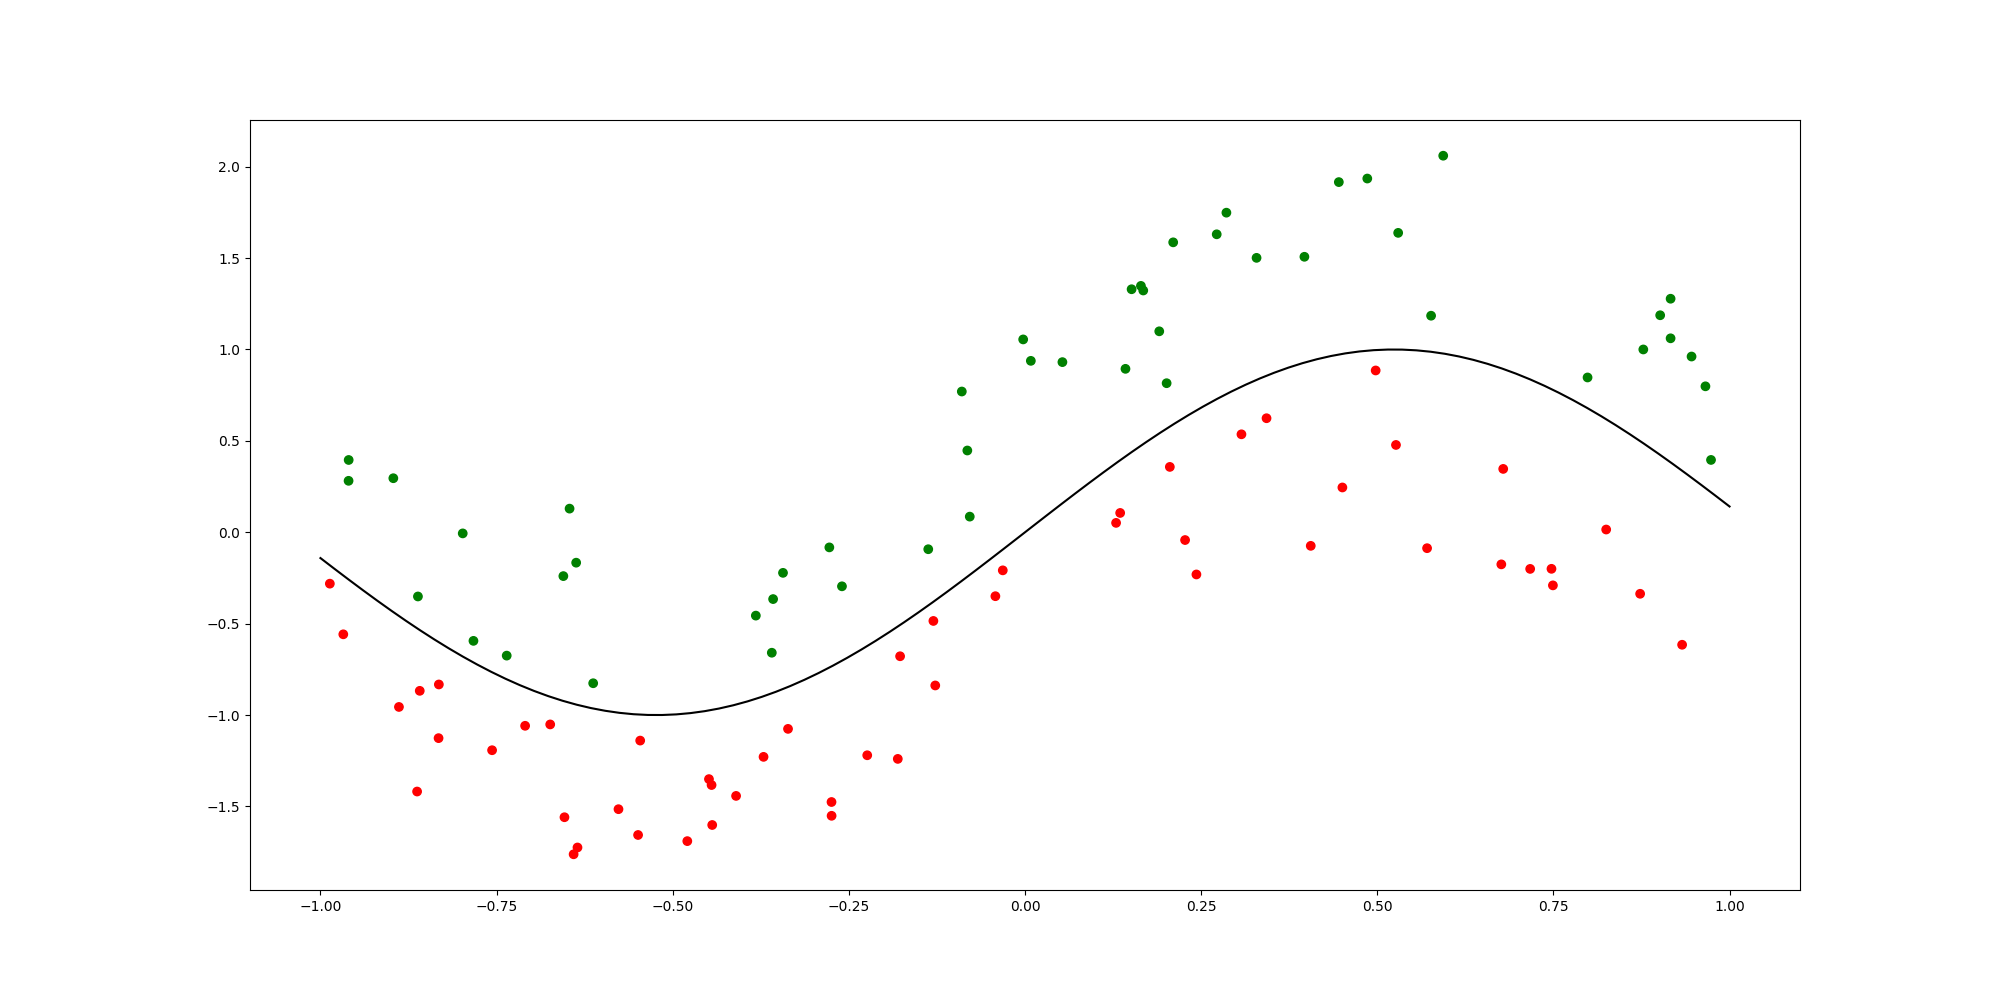
\includegraphics[width=\linewidth]{diagram2.png}
\end{frame}

\begin{frame}
    Machine learning techniques, specifically \textbf{binary classifiers}, can be used to deal with these situations.
\begin{enumerate}
\item For each candidate, we have a set of \texttt{Rosetta} scores \texttt{fa\_atr}, \texttt{fa\_sol}, ...
    These are called \textbf{factors}. Any candidate mutant is described by a vector of factors in a high-dimensional space:
    $$\vec{x} = (E_1, E_2, E_3, ..., E_m)$$
    
    \item Each candidate mutant is associated with its \textbf{class} $\in \{0, 1\}$. Here, 0 = 'non binding', 1 = 'binding'. We seek a map $F : \vec{x} \in \mathbb{R}^m \to \{0, 1\}$ that can predict \textbf{class} from \textbf{factors}.
    
    \item Machine learning methods allow approximations for such a function $F$ to be iteratively \textbf{learned} by a computer.
\end{enumerate}
\end{frame}

\begin{frame}
    Three binary classification approaches were employed, implemented in Python using \texttt{sklearn} library.
    \begin{enumerate}
        \item Logistic regression | linear model
    \item Artificial neural network (ANN) | nonlinear model
        \item Support vector machine (SVM) | nonlinear model
    \end{enumerate}

\end{frame}

\section{Methods}
\begin{frame}{Training set}
    Training set comprised of uAAs reported in a literature review to be incorporated by \textit{p}CNFRS mutant.
    
    Dumas et al., \textit{Chem. Sci.}, 2015, 6, 50 $\rightarrow$ 60 mutant-uAA pairs.
    
    uAA ligands were \textbf{chemically diverse.}
    
    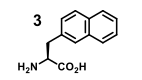
\includegraphics[scale = 0.4]{uAA3.png}
    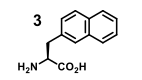
\includegraphics[scale = 0.4]{uAA5.png}
    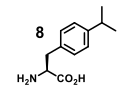
\includegraphics[scale = 0.4]{uAA8.png}
    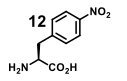
\includegraphics[scale = 0.4]{uAA12.png}
    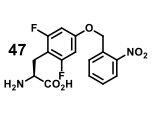
\includegraphics[scale = 0.4]{uAA47.png}
\end{frame}

\begin{frame}{Methods}
    \begin{itemize}
        \item Molecular models of uAA ligands constructed, 200 conformers generated using \texttt{balloon}
        \item Mutations modelled onto sequence of \textit{p}CNFRS (PDBID \texttt{3QE4})
        \item uAAs placed in aaRS binding cavity of \textit{p}CNFRS crystal structure using \texttt{pymol}
        \item Catalytic constraints manually specified for each mutant-uAA pair
        \item 500 candidate protein poses generated for \textbf{each} mutant-uAA pair using Rosetta \texttt{EnzymeDesign}
    \end{itemize}
    \begin{center}$\Rightarrow$ $(+)$ dataset!\end{center}
\end{frame}

\begin{frame}{Methods}
    For binary classification, using a \textbf{balanced} training dataset is important to avoid bias. Same protocol used to produce the following datasets:
    \begin{itemize}
        \item Mutants against uAAs $(+)$
        \item Mutants against Tyr $(-)$
    \end{itemize}
    \begin{itemize}
        \item Wt \textit{Mj}TyrRS against uAAs $(-)$
        \item Wt \textit{Mj}TyrRS against Tyr $(+)$
    \end{itemize}
    
    $\Rightarrow$ For each mutant-uAA pair, select top 10\% for ligand binding energy.
    
    $\Rightarrow$ Smaller datasets were randomly oversampled so all four datasets were of \textbf{equal size}.
    % Index([u'fa_rep', u'hbond_sc', u'all_cst', u'tot_burunsat_pm',
    %   u'tot_total_charge', u'tot_total_neg_charges', u'SR_13_fa_rep',
    %   u'SR_13_all_cst', u'SR_13_dsasa_1_2', u'SR_13_hbond_pm',
    %   u'SR_13_burunsat_pm', u'fa_atr_lig', u'fa_intra_rep_lig',
    %   u'atom_pair_constraint_lig', u'total_lig'],

\end{frame}

\begin{frame}{Implementation}
    Machine learning algorithms were implemented in \texttt{python} using the \texttt{sklearn} library.
    \begin{itemize}
        \item $k$-fold cross-validation is standard practice to measure classifier accuracy. Here $k = 5$
        \item Points were grouped with respect to mutant-uAA pair to prevent 'cheating'
    \end{itemize}
    
    \center\quad\quad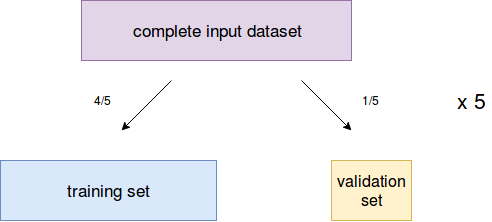
\includegraphics[width=0.6\linewidth]{CVdiagram.png}
\end{frame}

\section{Results and discussion}
\begin{frame}{Results and discussion}
    Optimal parameters were determined by grid search (not shown).\\
    Scores:
    \begin{itemize}
        \item \textbf{ANN}\quad 88.9\% (1 hidden layer);\quad 90.7\% (2 hidden layers)
        \item \textbf{SVM}\quad 89.1\% (RBF kernel)
        \item \textbf{LR}\quad 68.4\% ... :(
    \end{itemize}
    
    $\Rightarrow$ \textbf{binding} vs. \textbf{non-binding} distinction is \textbf{nonlinear!}
    $\Rightarrow$ \textbf{ANN} and \textbf{SVM} methods are similar in performance
\end{frame}

\begin{frame}
    \textbf{Example} 4:1 training:validation split (5-fold cross-validation)
    \begin{center}
    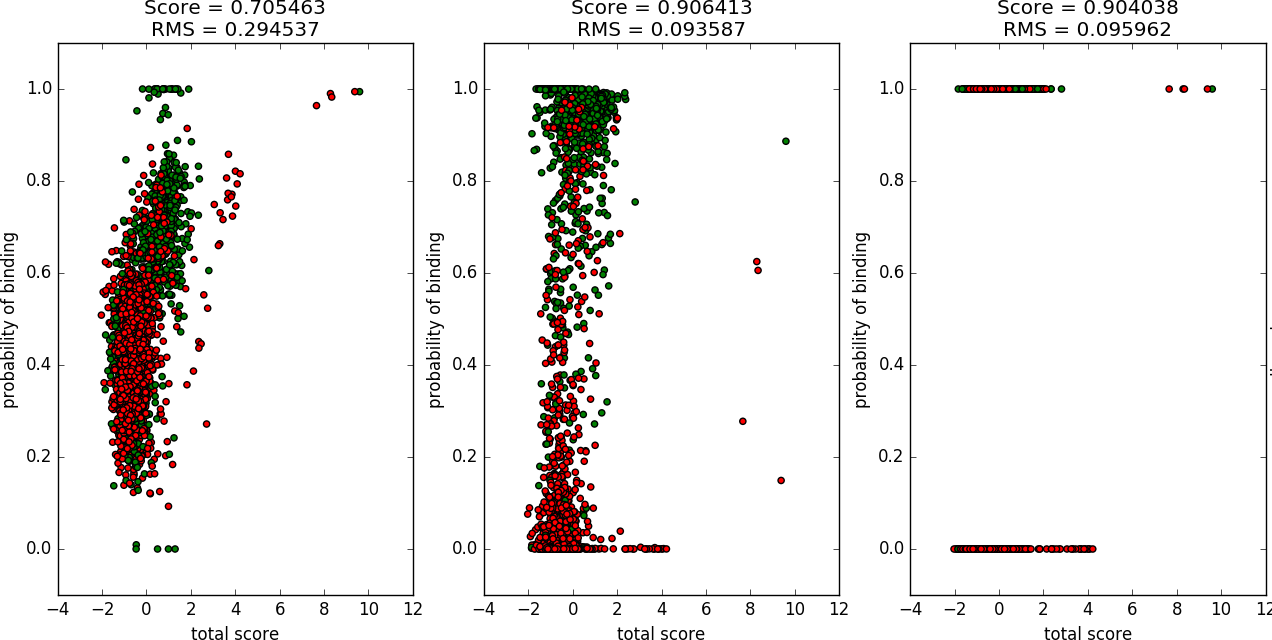
\includegraphics[width=\linewidth]{1-5split-classification.png}\\
    \hfill\textbf{Logit model}\hfill\textbf{ANN model}\hfill\textbf{SVM}\hfill\quad
    \newline
    \definecolor{darkgreen}{rgb}{0.0, 0.5, 0.13}
    \textcolor{red}{red = true negatives}\quad\textcolor{darkgreen}{green = true positives}
    \newline\newline\newline
    \end{center}
\end{frame}

\begin{frame}{Putting it to the test...}
\begin{itemize}
    \item \textbf{Nitroxide spin-label uAA} | 28 mutants | incorporation shown \textit{in vitro}
    \item \textbf{Bulk data scores}: LR 51.3\%; \textbf{ANN 82.3}\%; SVM 77.5\%
    \item \textbf{Individual mutants}: \textbf{ANN/SVM} 20/28 predicted to bind
\end{itemize}
\begin{center}
    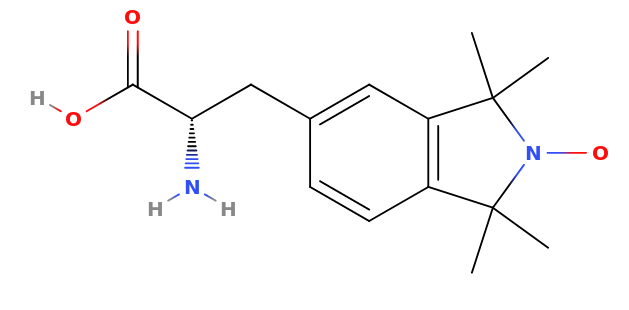
\includegraphics[scale = 0.2]{EPR.png}
\end{center}
\end{frame}

\begin{frame}{Mutant NF04}
    \begin{center}
    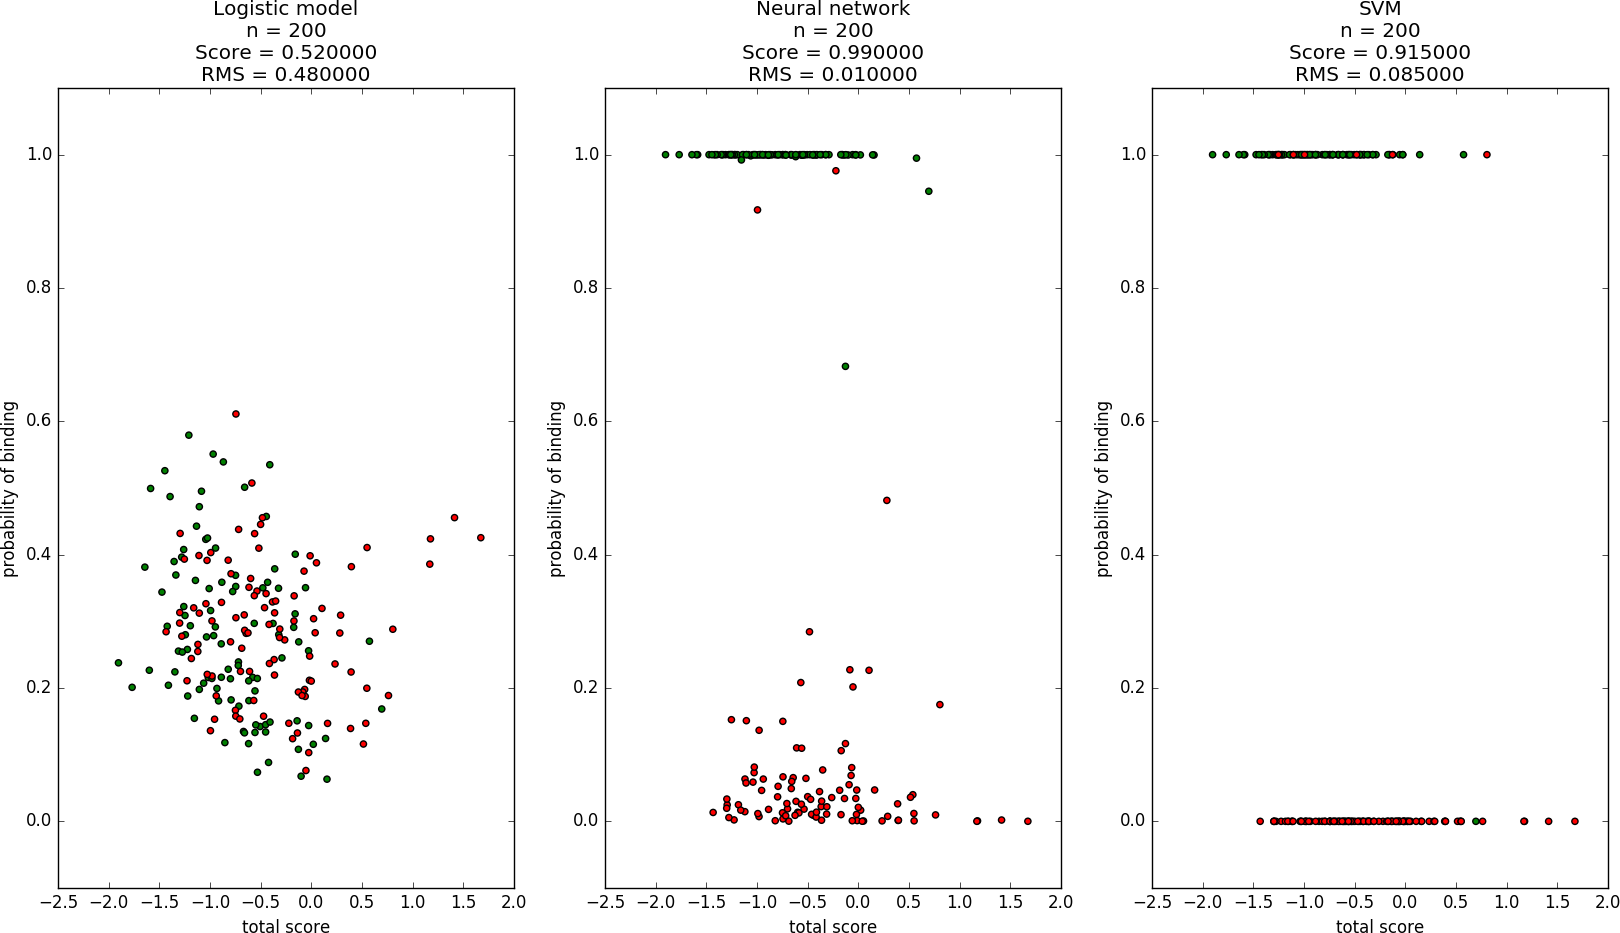
\includegraphics[scale = 0.23]{NF04_classif.png}
    \end{center}
\end{frame}

\begin{frame}{Putting it to the test...}
    Classifiers were tested on several \textbf{other} known mutant-uAA pairs
    \begin{itemize}
        % Coumarin 
        \item Schultz et al. (2011), \hfill\textbf{11/13} predictions correct\\
        %\hfill 6 known binding, 7 known non-binding
        \item Padilla et al. (2016), \hfill\textbf{1/2} predictions correct\\
        %\hfill 1 known binding, 1 known non-binding
    \end{itemize}
    
    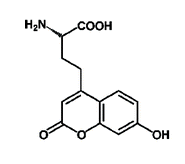
\includegraphics[scale=0.5]{coumarin_UAA.png}\hfill
    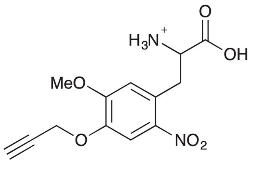
\includegraphics[scale=0.4]{Padilla_UAA.png}
\end{frame}
\begin{frame}
Introduce \textcolor{red}{sanity checks} where aaRS is known to bind \textbf{natural} amino acids...
    \begin{itemize}
        \item Phe-incorporating \textit{p}CNFRS mutant (NAA03) predicted correctly.
        \item \textit{Mj}TyrRS shown to bind to Tyr and not uAA from Padilla et al.
    \end{itemize}
\end{frame}

\begin{frame}{Mutant NAA03 (Phe incorporating \textit{Mj}TyrRS mutant)}
    \begin{center}
    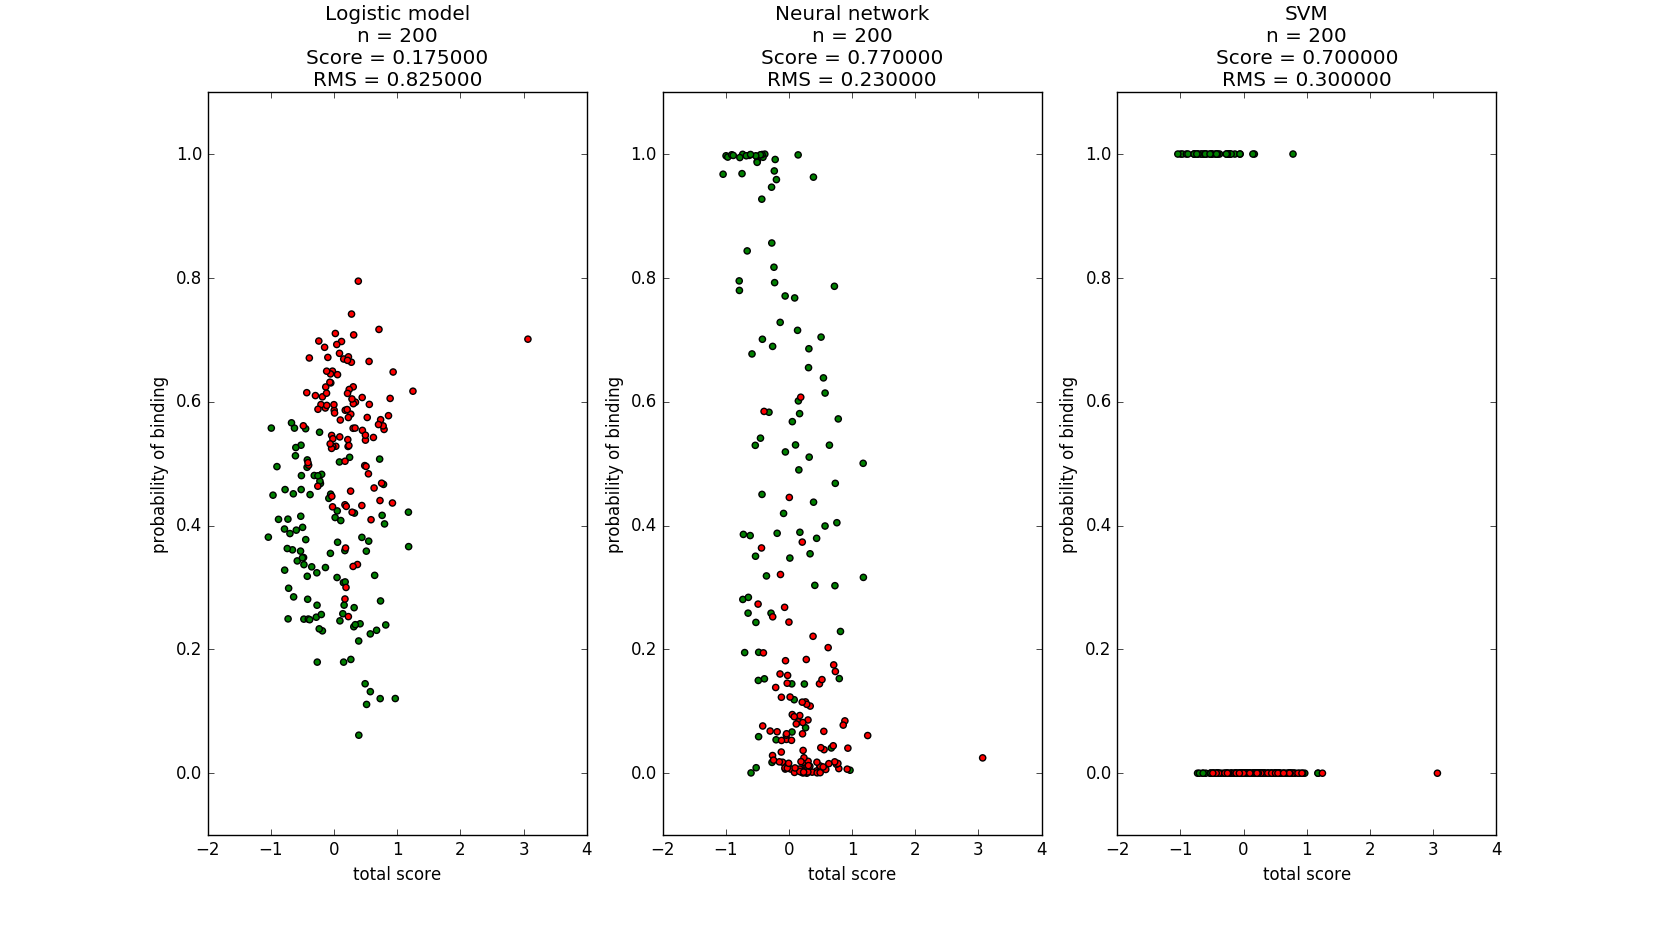
\includegraphics[scale = 0.23]{NAA03_classif.png}
    \end{center}
\end{frame}

\begin{frame}{Summary}
    \begin{itemize}
        \item Machine learning techniques can be applied to screen for 'hits' in computational protein design
        \item Performance is \textbf{critically dependent} on a broad and high quality training data
        \begin{itemize}
            \item Mitigated in part by inclusion of wt aaRS data, but \textbf{much to be desired}
        \end{itemize}
        $\Rightarrow$ hopefully we can get some better data in future!
    \end{itemize}
    
    \begin{center}\textcolor{red}{garbage in $\Rightarrow$ garbage out}\end{center}
\end{frame}

\begin{frame}{Acknowledgements}
\begin{itemize}
    \item \textbf{Prof. Thomas Huber}
    \item Haocheng Qianzhu
    \item Abera Saeed
    \item Youssef Latash
\end{itemize}

Research School of Chemistry, ANU

NCI (much needed computing time)

\end{frame}
\end{document}


